

\setcounter{section}{5}
\section{Software Design}
\bigskip

% NOTE: future work would be to build a system to flash new beacons with firmware for the credentials to communicate with the system.
% NOTE: assume beacons have line of sight to eachother. this allows us to make the callibration phase easier by manually measuring the distance between beacons rather than creating a callibration script.

%Libraries/Packages/Frameworks
%Software Stack

% discuss the system at a high level, but leave details to subsections
% breifly reintroduce important topics that the user will need to be reminded of
\subsection{Software Overview}
% TODO revise
The Akriveia system is comprised of 3 different devices, namely: the data processor, beacons, and ID tags; this device diversity plays a large role in the software choice for the beacons and id tags.
\smallskip
The Akriveia data processor is the primary access point for Administrators and First Responders, of whom will be presented a Graphical User Interface served by the data processor in addition to handling commands from the client.
The software on the server is written entirely in Rust, including the static client side webpage.

\smallskip
The requirements for each device are different, however the id tags and beacons are able to share a similar environment.
As such Akriveia will require two different software environments.

\bigskip
% language choices, formatting, standards, libraries
\subsection{Software Stack}
Akrivia is composed of two primary languages, the server is implemented entirely in Rust while the beacons and ID tags use C++.

\bigskip
\subsubsection{Software Environments}
The data processing server requires an operating system to perform mundane CPU scheduling for our multithreaded application, wifi drivers, and a proper file system to handle a database.
As such, the linux - and more specifically the debian destribution of linux - was chosen as the servers operating system.

\bigskip
% TODO add a citation for debian stability
Debian is widely praised for its stability, which makes it ideal for a data processing server because Akriveia simply cannot fail as lives depend on it to work.
Debian brings in the aptitude package manager for dependency management, which allows for quick installation of required driver updates, operating system updates, and any additional packages required by Akriveia.
Debian's Aptitude has the advantage compared to other package managers because it removes the need to worry about dependencies, manual installation, and even installation of sub dependencies.
As Debian is a linux distribution, it has widespread hardware adoption across many different hardware architectures - primarily x86-64 and ARM64 - giving Akriveia the flexibility to run almost anywhere with little cost.

\bigskip
Debian is contrasted by another linux distribution called arch linux which uses a different package management paradigm called rolling releases, favoring earlier adoption of newer packages to more quickly introduce features at the cost of stability.
Another alternative to Debian is Windows, however Windows suffers from high power usage, poor package management, and heavy reliance on proprietary software, whereas linux is free of cost, open source, and has a more inclusive licence.

\bigskip
\subsubsection{Software Languages}
% TODO revise with word flow in mind. segmented thoughts in each sentence.
The server is written in Rust.
% TODO make the citation work
Rust is a newer language compared to C, it was created in 2006 \cite{rust_graydon_interview} and its first stable version was released in 2015 \cite{rust_releases}, taking inspiration from C++ and Haskell in its design.
Rust is a systems language designed for stability and robustness, it eliminates entire classes of errors using its borrow checking system, a feature unique to this language.
The borrow checking system defines a strict set of rules to follow, and fails to compile if these rules are broken - even if the application is otherwise logically correct.
As a systems language, Rust is compiled to binary rather than executed as a script through an interpreter however this does not stop it from being a higher order language.
The borrow checker statically analyzes the code being compiled, and in doing so is able to statically determine when to allocate and more importantly when to free heap allocated memory.
Fundamentally, this means that without a garbage collector and without manually managing memory, Rust provides a mechanism to manage memory without a runtime cost while behaving like a garbage collected language providing great flexibility in expressiveness and allowing higher order operations without taking brain resources.

\bigskip
The beacon and id tag are written in C++.
Ideally, the entire project would be written in one languge, however for the case of programming embedded devices, namely arduinos, we have opted to stick wih the standard toolset shipped with the arduino tools.
C++ is specifically designed for embedded programming, allowing use of higher level features when desired while also giving the developer absolute control over how memory is managed.
On arduinos, memory is very limited so control is key to fitting our program within the small space constraints.


\bigskip
\subsubsection{Software Standards}
% TODO references here
Rust code will follow the the Rustfmt standard of source layouts, Rustfmt is a tool provided by the Rust project that automatically formats all source in the standard format. The Rust compiler also provides a few warnings for common formatting issues builtin, which will be heeded.

\bigskip
C++ will follow the iso C++ programming standards \cite{cpp_core_guidelines}. The arduino style guide \cite{arduino_style_guide} was also considered, however the rules list they present is incomplete and more ad hoc than a full style guide.

% introduce major libraries that largely dictate how we implement the system.
\subsubsection{Frameworks}
Akriveia's main server framework is called Actix.
Actix is an Actor Framework that follows the Actor Model paradigm of multithreaded workloads.
The Actor Model operates on objects called actors to orchestrate concurrent computations, it does this by treating actors as seperate entities that execute on an event loop on one or more threads, where the event loop simply looks at a list of events generated by actors and executes each event in order as long as it is not blocked by other events.
Events are generated when actors pass messages to eachother, in response the actor that receives the message can modify its local state, create other actors, send messages to other actors, execute arbitrary logic, and finally send a response to the message.
This programming paradigm prevents the need for locks (and by extension, deadlocks) because the message passing mechanism alleviates the need to manually manage concurrency, opting to use atomics instead.
\bigskip
Actix was chosen as the primarily to give the flexibility of multithreading without incurring the typical thought process overhead associated with multithreading. Additionally, as a framework rather than a library, Actix serves as the basis to make REST webservers through the package Actix Web, which is further discussed under the \ref{software_libraries} section.

% discuss which libraries we are using, and how they will be used by us
\subsubsection{Libraries}
\label{software_libraries}

\begin{table}[H]
\centering
\begin{tabular}{ | m{3.25cm} | m{12.5cm} |}
	\hline
	\textbf{Actix Web} & The Actix Web library is a crate that extends the functionality of the Actix framework to create HTTP webservers. \\
	\hline
	\textbf{Yew} & Yew is a crate that extends Rusts ability to compile to Web Assembly by adding the ability to dynamically generate html on the client in response to user events and server responses. This library is very similar to Facebook's React for javascript. \\
	\hline
	\textbf{Serial Port} & Enables serial communication over USB between the server and beacons.\\
	\hline
	\textbf{Rust Standard Libraries} & This is the standard Rust runtime library, and contains many useful boilerplate functions and generic types. This library is included with the basic installation of Rustc. \\
	\hline
\end{tabular}
\caption{Akriveia Dependencies - Rust}
\end{table}

\begin{table}[H]
\centering
\begin{tabular}{ | m{3.25cm} | m{12.5cm} |}
	\hline
	\textbf{Arduino Runtime} & This is the standard set of arduino runtime libraries based off of the clib standard library tailored specifically for Atmel Atmega microcontroller chips. \\
	\hline
	% TODO wifi library
\end{tabular}
\caption{Akriveia Dependencies - C++}
\end{table}

\bigskip
% discuss the model view controller paradigm, and its benefits
\subsection{Model-View-Controller}
% TODO glossary of mvc
The model-view-controller(MVC) paradigm is a common method of seperating concerns between modules.
It is an architectural pattern that seperates concerns in a general way, allowing for code reused and improving parallel developement, it is also a common practice which allows others familiar with the paradigm to ramp up quickly on the project.
The model describes data, data manipulation, as well as data storage.
The view simply describes how to view the model.
The controller acts as the means to communicate between the view and model based on data inputs, and is also capable of higher order operations such as between multiple models.

\bigskip
As the Actix Web library is less mature than frameworks in other languages such as Python's Django or Ruby's Rails, Akriveia's data processor will be an implementation of a large portion of manual MVC boilerplate.
This allows for greater flexibility in implementation, at the cost of marginally higher developement time.
A benefit is that MVC does not have a good answer for funcitonality that falls outside of the architectures coverage such as background tasks.
Akriveia is required to maintain communication with many beacons and perform calculations asyncronously from web requests, which is the perfect usecase for the actor framework which fills the void of the model-view-controller.


\bigskip
% discuss how we plan to multithread the data processor. go into slightly more detail about actix actors, and why this
% is necessary
\subsection{Threading Model}
The purpose of multithreading the DPU is to make use of the hardware provided, since all modern server and desktop processors have at least two dedicated hardware cores.
Additionally, it is important for the DPU to have realtime responsiveness on the webserver, requiring that large computations such as triangluation for many beacons must be offloaded to other threads, keeping responsiveness high since the webserver thread is not blocked on computation while a request comes in.
An additional consideration specifically for the proof of concept which uses blocking serial communication to communicate to the beacons, meaning that each beacon requires a dedicated thread to communicate with the DPU.

Rust and Actix make multithreaded development easier by using message passing for interthread communication, at the cost of performance when compared to traditional mutexes and atomics.
The implementation of message passing is a thread safe queue using mutexes and atomics to ensure data integrity, where multiple threads are able to send commands to another thread, which recieve the message without blocking either thread.
To further discuss the Actix threading model, some definitions are required:
\begin{enumerate}
	\item Actor: A class that contains message handler callbacks.
	\item Arbitor: A thread pool, where each thread in the pool is an event loop.
\end{enumerate}
Once instantiated, the arbitor spawns as many threads as indicated by its constructor and waits for actors to be spawned within the thread pool.
By default, the number of threads in the pool is the number of cores on the CPU.
The arbiter is an environment for actors to execute, and as actors are spawned into the thread pool, they can send messages to other actors, or create other actors in response to external events such as from the file system or HTTP requests.
As shown in Figure~\ref{actix_thread_model}, the arbitor manages its own threads, which are all spawned at startup rather than on demand.
Within each thread, the arbitor executes the event loop, which polls its queue, and acts on any messages in the queue by delegating the task to the actor the message is bound to.
To pass a message to another actor, the sender must have the address of the recipient so that the arbitor can determine the destination, rather than a broadcasting system; this is shown in Figure~\ref{actix_messages}.

\begin{figure}
	\centering
    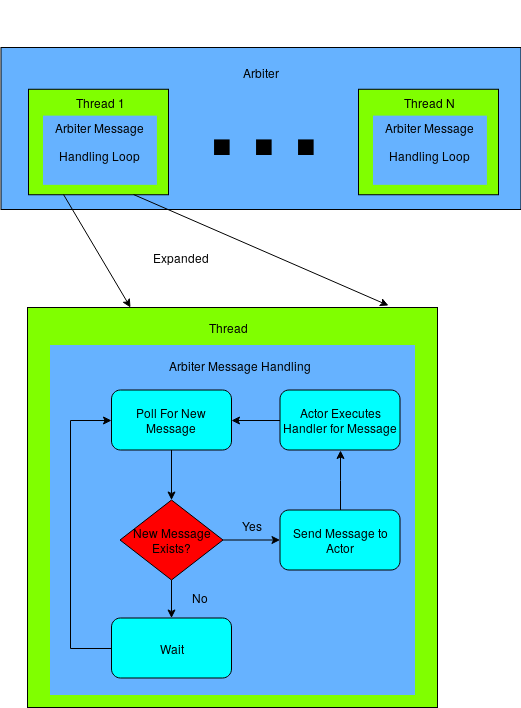
\includegraphics[scale=0.6]{images/actix_thread_model.png}
    \caption{Actix Thread Model}
    \label{actix_thread_model}
\end{figure}
\begin{figure}
	\centering
    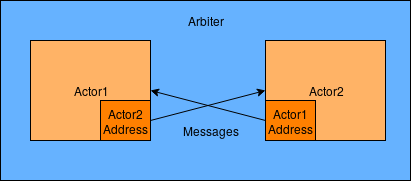
\includegraphics[scale=0.6]{images/actix_message_passing.png}
    \caption{Actix Message Passing}
    \label{actix_messages}
\end{figure}

The beacons and ID tags do not have a full operating system, so they can only rely on single threaded interrupt handling to "multitask".
Interrupt handling does not provide full concurrency, instead it time slices the single core to provide the illusion of multitasking.
Interrupt handling is calling a function as a result of an event such as an external device raising a bit high on the CPU, or when a timer goes off.
In the Proof concept, the bluetooth library uses this functionality to handle connections.
When transitioning to wifi and UWB, similar functionality will be implemented in each respective technology's library, of which Akrievia simply relies on rather than reimplementing ourselves.

\bigskip
% discuss the data processor subsystems in detail
\subsection{Data Processor Software Architecture}
In the proof of concept, the DPU creates an HTTP server actor and a beacon manager actor.
The HTTP server waits on web requests, delegating tasks to the beacon manager and polling it for the necessary information.
On startup, the beacon manager queries the number of serial arduino devices, spawning a thread for each device.
Each thread spawned by the beacon manager represents a serial connection to a beacon.
The beacon manager sends messages using a traditional Multiple Producer Single Consumer Message Queue (MPSC) defined in the Rust standard library, while the each serial communcation thread returns messages back to the manager through the actix message passing system.
Figure~\ref{software_poc_arch} gives a graphical representation of the previous description.
As a side note, Actix uses MPSC internally for its message passing system.

\bigskip
The prototype and final versions bring in major changes to the software design.
As shown in figure~\ref{software_final_arch}, a major change is the removal of the serial connection actor which is replaced with the udp actor(which tentatively may be tcp instead).
The beacon manager remains, but instead controls the udp actor rather than the serial connections.
An additional role of the beacon manager is to delegate computation of triangulation to the triangulation processor actor, which will save data in memory until there are at least 3 data points for a single it tag to determine its position.
The triangluation processor makes the positional calculation and saves new position to disk via the id tag model, which abstracts the database query.
The beacon and map models perform a similar role, abstracting their associated database queries into a single location following MVC.
Controllers mainly handle the model they were paired with, however the id tag controller will also query the triangulation processor for realtime positional data and the beacon controller commands beacons indirectly through the beacon manager.

\bigskip
By design, the DPU is a client-server architecture, where the DPU is the server for a browser based client.
The client-server architecture lends itself to be very flexible and is a very heavily used model for both consumer systems and emergency response systems alike.
Once the backend starts executing, any computer able to access the IP of the DPU will have access to our system assuming the network is configured in such a way to allow this, conversely with no additional developement work the same server when hooked up to a monitor can act like a client based application by simply accessing localhost on a browser.
A client-only application lacks this deployment flexibility.
Variations and alternatives to the client server-architecture were considered, but did not meet the needs of Akriveia, below are some of the choices considered and why they do not fit the role.

\bigskip
An electron application that utilizes browser technologies merges the backend and frontend together, behaving like a client based application, which will reduce deployment flexibility because a monitor connected directly to the DPU will be the only access point to the GUI, however the display will potentially need to be accessed by multiple users at a time, and will introduce high coupling between the frontend display and backend computation.
Electron applications are also highly single threaded, meaning that they will have higher difficulty in utilizing all cores on the CPU, wasting money on hardware that could otherwise be used.
Electron applications are also fixed to using a single language, Javascript, for both processing and display, whereas a webserver fixes the GUI implementation to Javascript however leaves the backend to a mucher broader range of languages where processing power is required.

\bigskip
Compared to a GUI implemented using graphics driver interfaces such as OpenGL, Vulkan, DirectX, or any higher level libraries that provide interfaces to graphics drivers, a GUI implemented in HTML and Javascript will take much less time to implement because both Javascript and HTML abstract away memory concerns such as pointers, and will never have memory related runtime errors, as guaranteed by the browser.
Browsers have widespread adoption, in every GUI based operating system at least one browser is installed by default, making them widespread and widely used.
Due to widespread adoption, browsers provide the flexibility to display our GUI either on the computer hosting the server itself, or just as easily the GUI can be accessed through another computer at the customers discretion.

\begin{figure}[H]
	\centering
    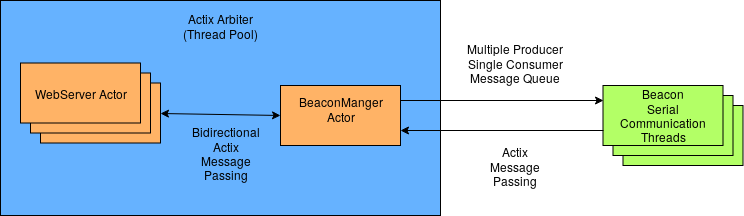
\includegraphics[scale=0.6]{images/poc_arch.png}
    \caption{Proof of Concept Software Architecture}
    \label{software_poc_arch}
\end{figure}

\begin{figure}[H]
	\centering
    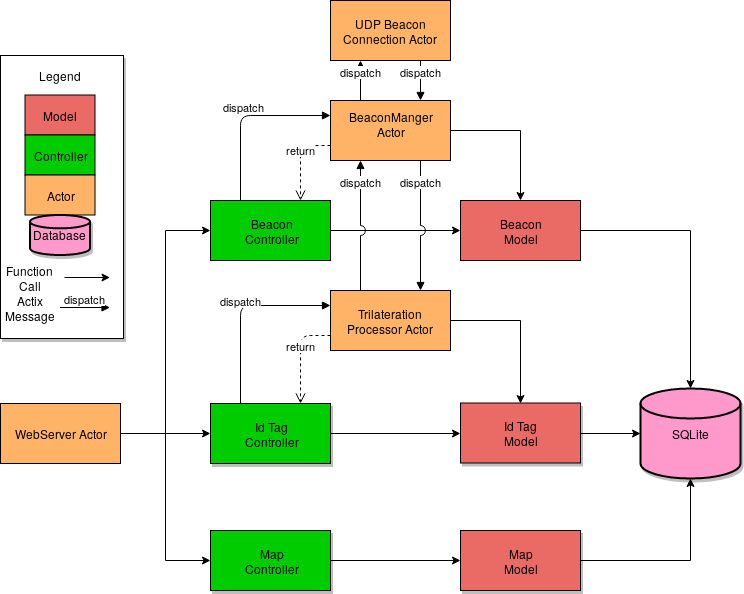
\includegraphics[scale=0.6]{images/prototype_software_arch.png}
    \caption{Final Software Architecture}
    \label{software_final_arch}
\end{figure}

\bigskip
% discus the purpose of the webserver, and how it will be used to control the other subsystems dictated by user command.
\subsubsection{Webserver Subsystem}
The purpose of the Webserver Subsystem is to bridge the GUI and backend by providing a data transfer interface in the form of HTTP REST calls.
A Webserver architecture is chosen because of its simplicity to implement, widespread adoption, and flexibility.
The view is discussed further in Section~\ref{view_section}.

\bigskip
The Webserver Subsystem will be designed to serve data to a browser, including the the HTML and Javascript files(GUI files) that are displayed by the browser.
Once the browser has the GUI files, it will make addiitonal requests to the backend to keep updated information displayed on the GUI.
The Webserver Subsystem will only allow logged in users to access sensitive data, and only if they have the correct access rights.
Electron applications and traditional rendering APIs were also considered, however they each have tradeoffs that do not fit with the design requirements of Akrievia.

\bigskip
A direct alternative to Actix Web is a web framework called Rocket.
Rocket behaves more like a traditional web server: supporting server side rendering and json parsing out of the box.
This functionality comes at a cost in multiple ways, first rocket is primarily single threaded, second Rocket adds new features at the cost of reducing flexibility, and third rocket does not directly support the Actix Actor system, leaving all non-webserver code up to the developer to implement on their own.
In comparison, Actix Web does support and extend the Actor system which makes for a more integrated and unified codebase, and by using the Actor system within the webserver, multithreadability is easily added as needed on a per endpoint basis.
Rocket's additional out-of-the-box features are really just Rust crates in disguise, and so by using Cargo(Rusts package manager for crates) the same functonality can be quickly implemented within an Actix webserver at very little additional time cost.

\bigskip
\subsubsection{Beacon Manager Subsystem}
The role of the beacon manager is to aggregate data from the individual beacon connections, and to give an abstraction for external systems that need not concern themselves with communication details, or how many beacons there actually are.
The Beacon Manager is a singleton, which means there is only one of them in the entire system, and has implications on the design of the rest of the system.
The most notable design influence is that the beacon manager can quickly become a bottleneck if it performs too much processing directly, and so to prevent this the beacon manager offloads as much work as it can to other subsystems.

\bigskip
\subsubsection{Serial Beacon Communication Subsystem}
In the proof of concept design, this actor deals with blocking serial communication with dedicated threads to keep the connection alive and to prevent web requests from blocking.
This subsystem will remain as bare bones as possible, because it only serves the purpose of quickly creating a working system and will likely be discarded in future iterations of the DPU.

\bigskip
\subsubsection{Triangulation Processing Subsystem}
In the final design, the triangulation processing subsystem takes in RSSI and time of flight messages from the beacon manager.
The triangulation processor waits until it receives enough datapoints, and once it has 3 datapoints from 3 different beacons for one id tag it can perform a location calculation
While waiting for a full set of data, the incomplete set of data will be stored in a hash table where the mac address of each ID tag is the key and the contents are an array of data points.
Once the array of datapoints hits the threshhold size of 3 from adding a new datapoint the processor can perform the full triangulation calculation.
The triangulation calculation can then be used to update the database entry for the corresponding ID tag by the processor.
To avoid going to the database for realtime updates of the ID tag locations, the ID tag controller will directly query the Triangulation Processor for the most up to date location infromation, reducing latency.

The existance of the Triangulation Processing subsytem is necessary, because the beacon manager will quickly become a bottleneck due to the fact that it is a singleton in a multithreaded system.
As such, the manager should do as little direct processing and blocking operations itself and instead favor offloading the tasks to other subsystems.

\bigskip
\subsubsection{UDP Beacon Communication Subsystem}
In the final design, this actor will communicate with the beacons over the UDP networking protocol.
UDP was chosen because it has less overhead than TCP, and is more suited for realtime applications such as Akriveia.

\bigskip
% discuss database choice - sqlite and why. lead into our models
\subsection{Database}
Akrievia requires a database to persist map, beacon, and user information.
In the time constraints of Capstone, the database will be a central location for data.
Ideally a production system would support replication of the database to another location, but this is out of scope for the purposes of this course.

\bigskip
SQLite was chosen primarily because of its simplicity to setup and minimal footprint.
Most commonly used in phones and packaged alongside python, SQLite has a stable file format and large userbase, and because of this has built a reputation for not failing.
SQLite is open source, and because of this issues can directly be brought up to the developers along with help from a large amount of experience from the internet due to the large userbase.
Open source projects are also freely available to browse to learn directly from the codebase when necessary.
In Akriveia, the database is accesed through model objects to keep concerns local to a single set of similarily structured files, and to keep reusability up in the codebase.

\bigskip
% discuss how we plan to represent data in the database, tie back to model-view-controller(specifically models, which
% will implement all of the database queries for the controllers to use.
\subsection{Models}
Models are used to group database queries and model operations into a single file for each model, increasing reusability of the system.
Akrievia is expected to maintain three different types of models: maps, ID tags, and beacons.
The following tables \ref{user_model}, \ref{beacon_model}, and \ref{map_model} show expected data entries and their type for each model, along with the purpose of each entry.

\begin{table}[H]
\centering
\begin{tabular}{| m{3cm} | m{3cm} | m{9.5cm} |}
	\hline
	\multicolumn{3}{|c|}{User Model} \\
	\hline
	Data Name & Type & Explanation \\

	\hline
	Coordinates & 2D Vector & Last known location of the user within the map. \\
	\hline
	Emergency Contact & ref:User & Reference to another user as an emergency contact. emergency contacts wont have an employee id or tag id. \\
	\hline
	Employee Id & String & Employee id for each user, optional, may be useful for internal housekeeping of the company that purchases Akriveia. \\
	\hline
	Full Name & String & Human readable name to identify the user on lists. \\
	\hline
	Id Tag Number & 64bit Integer & table key, unique, id for each user. \\
	\hline
	Last Seen Timestamp & Unix Timestamp & Helps to identify if the id tag data is stale. Used to determine if the employee is at work while the disaster occurs. \\
	\hline
	Map ID & ref:Map & Last known map the user was located at. \\
	\hline
	Notes & String & Notes about the user, ie allergies or disabilities, etc. \\
	\hline
	Phone Number & String & Phone number to contact the user. \\
	\hline
	User Type & String & Indicates the type of user, either admin, employee, emergency contact, or first responder. \\
	\hline
\end{tabular}
\caption{User Model}
\label{user_model}
\end{table}

\begin{table}[H]
\centering
\begin{tabular}{ | m{3cm} | m{3cm} | m{9.5cm} |}
	\hline
	\multicolumn{3}{|c|}{Beacon Model} \\
	\hline
	Data Name & Type & Explanation \\

	\hline
	Mac address & String & unique device identifier for beacon, table key.\\
	\hline
	Map id & ref:Map & Reference to a floor/map - this is really just the floor number. Shows the many-to-one relationship between beacons and floors. \\
	\hline
	Name & String & Human readable String for the device. \\
	\hline
	Notes & String & Notes for the beacon such as which room the beacon is located at. \\
	\hline
\end{tabular}
\caption{Beacon Model}
\label{beacon_model}
\end{table}

\begin{table}[H]
\centering
\begin{tabular}{| m{3cm} | m{3cm} | m{9.5cm} |}
	\hline
	\multicolumn{3}{|c|}{Map Model} \\

	\hline
	Data Name & Type & Explanation \\
	\hline
	Name & String & Human readable floor name for gui. \\
	\hline
	Floor number & String & Table key, unique floor number of the map, this is not an integer to accomodate the possibility of odd floor naming conventions. e.g. floor 1A, or basement. \\
	\hline
	Bitmap data & Binary & Bitmap for the floor blueprints to view on the gui. \\
	\hline
\end{tabular}
\caption{Map Model}
\label{map_model}
\end{table}


% discuss what each controller will do - i dont expect this one to be very meaty
\subsection{Controllers}
Controllers are part of the MVC philosophy, unfortunately actix does not directly support the idea of controllers, however this functionality can be implemented manually using Actix Web primitives.
Each controller exposes available operations for the frontend to manipulate data in a controlled and secure manner.
The controller manages data using the models to perform direct manipulations and can aggregate data that cannot otherwise be done by models.
Table~\ref{controllers_table} shows the list of expected controllers in the DPU, one to match each model.

\begin{table}[H]
\centering
\begin{tabular}{| m{3cm} | m{9.5cm} |}
	\hline
	\multicolumn{2}{|c|}{Map Model} \\
	\hline
	Controller Name & Explanation \\
	\hline
	Maps & Handles requests for map operations such as to create, update, delete the map instances. \\
	\hline
	Beacons & Handles requests for beacon operations such as to create, update, delete beacon the model instances. \\
	\hline
	Users & Handles requests for user(id tag) operations such as to create, update and delete user instances. \\
	\hline
\end{tabular}
\caption{Controllers list}
\label{controllers_table}
\end{table}

% describe how the view will work, but dont go into details about the GUI visuals - leaving that for the ui appendix
% mention browser, js, html, Rust -> webassembly compile
\subsection{View}
\label{view_section}
The view is part of the MVC philosophy.
The job of the view is to display data in a friendly and easy to use GUI.
In Akriveia, the view is a static webpage served by the Actix Webserver, and is compiled seperately from the backend.
Traditionally, the browser would render HTML and Javascript served by the backend webserver, however in this project the frontend is written entirely in Rust and compiled to a small HTML stub and webassembly which then dynamically generates more HTML for the browser to render.
The Yew crate makes this all possible, which is a Rust package that leverages the webassembly LLVM backend for Rust.
Yew is influenced by Facebook's React, a widely used Javascript library to generate dynamic webpages.

\bigskip
As Yew is influenced by React, it is very possible to simply write the GUI using React.
The drawback to using React is that it is written in Javascript, meaning that an implementation using React would make the language of the backend different from the language of the frontend, incurring overhead when developing.
An additional drawback to using React is that struct definitions and interfaces would need to be implemented twice, once in each language, adding tedious boilerplate.
The modern Javascript development environment as a whole is also getting fairly unweildy, as of 2019 more packages are being added which each introduce transformation steps of the code.
An example of this workflow could involve writing typescript which is transformed into Javascript, then minimizing the Javascript into unreadable but more performant minimized Javascript.
Additional steps would similarily be added for babel scripts.
In the example both of the steps are added to the build manually using webpack which incurs more development overhead to understand and configuration.
Yew on the otherhand has a opaque compilation step that transforms Rust code into webassembly, which does not require any additional build steps to configure other than installing the package.
One of the downsides to using Rust compiled to webassebly is that it simply cannot be debugged since it is more similar to binary, but this issue has not arisen yet since framework is very simple to use.
It does seem, in theory, possible to compile Rust to Javascript which can be debugged in the browser, but debugging Javascript which was generated from another language will likely not be a very fruitful exercise.

\bigskip
Server Side rendering of templates using libraries such as Askama and Tera were also considered instead of creating a single page website.
This method of rendering is fantastic for form submissions, however realtime and dynamic pages strain the abilities of server side rendering.
Akrievia will require realtime updates of maps, which will look and perform much better when rendered on the client side rather than having the backend needlessly rerender the same page with different data.
Typically, when realtime functionality is required for server side rendered applications, some pages are converted to using client side rendering while others remain server side rendered, requiring libraries like React or JQuery.
By simply using client side rendering, the frontend is consistenly implemented throughout, rather than requiring more than one type of rendering.

\bigskip
Please see the UI Appendix for additional details on the UI layout.

% discuss security considerations, talk about features of Rust which help us in this regard.
\subsection{Security}
Due to the properties of Rust, many security concerns regarding bad input data and memory issues are mitigated.
One such migitation is built in bounds checking of all array accesses, meaning that its not possible to read or write memory that has not been properly allocated by the executing process.
An additional level of security is that rust reduces the number of invalid computational state, removing the burden from the programmer which could potentially get it wrong, which would create vulnerabilities.
As rust is a strongly typed language, it also benefits from static type checking which eliminates entire classes of bugs that also could lead to vulnerabilities.

\bigskip
All stored user data will be encrypted using the latest encryption algorithms, namely the sha3-512 algorithm.
In memory data will be unencrypted for as short of a time as possible to reduce the surface area of potential attacks.

\bigskip

% TODO flesh these out into paras
functions of each beacon
	- sending data to the data processor
	- responding to commands from the data processor and acting on them
	- store data on each id tag encountered in an hash table entry - use the mac address as the key
	- store a rolling buffer for each id tag so that data points can be averaged, reducing error
	-

\bigskip

% TODO flesh these out into paras
functions of each id tag
	-




\pagebreak
\subsection{Software Design Requirements}
